\documentclass[12pt]{article}
\usepackage[utf8]{inputenc}
\usepackage[T1]{fontenc}
\usepackage{lmodern}
\usepackage{geometry}
\geometry{margin=1in}

\usepackage{amsmath, amssymb, amsfonts, bm, mathtools, empheq}


\usepackage{gensymb} 
\usepackage{siunitx}
\usepackage{physics}
\AtBeginDocument{\RenewCommandCopy\qty\SI} 

\usepackage{float}
\usepackage{caption}
\usepackage{subcaption}
\usepackage{booktabs}

\usepackage{setspace}
\usepackage{enumitem}
\usepackage{titlesec}
\usepackage{fancyhdr}
\usepackage{xcolor}
\usepackage[nottoc]{tocbibind}  

\usepackage{hyperref}
\hypersetup{
    colorlinks = true,
    linkcolor  = blue,
    citecolor  = blue,
    urlcolor   = blue,
    pdfauthor  = {},
    pdftitle   = {Modeling Temperature-Dependent Viscosity Effects in Crude Oil Pipeline Transport}
}



\title{Modeling Temperature-Dependent Viscosity Effects in Crude Oil Pipeline Transport: A Transport-Phenomena Approach}
\author{Under the guidance of Prof Vikrant Saxena}
\date{November 2025}

\pagestyle{fancy}
\fancyhf{}
\fancyhead[L]{\textit{Modeling Temperature-Dependent Viscosity Effects}}
\fancyhead[R]{}
\fancyfoot[C]{\thepage}

\setstretch{1.2}
\usepackage{tikz}
\usepackage{pgfplots}
\pgfplotsset{compat=1.18}
\usetikzlibrary{arrows.meta, positioning, calc}


\begin{document}
\begin{titlepage}
    \centering

   
    \includegraphics[width=4cm]{download.png}\par\vspace{1cm}
   

    
    {\Huge \textbf{CLL110 TERM PAPER}\par}\vspace{1.5cm}

    
    {\Large
    Abhinivesh Bajpai (2024CH70306)\\[0.3cm]
    Suhani Gupta(2024CH70291)\\[0.3cm]
    Lakshya(2024CH70624)\\[0.3cm]
    Khushi Kataria(2024CH70165)\\[0.3cm]
   
    }

    \vfill


   

\end{titlepage}


\maketitle
\thispagestyle{plain}

\begin{abstract}
Viscosity in heavy crude oils exhibits strong temperature dependence, making accurate prediction of temperature effects on the flow essential for efficient pipeline transport.  
In this work, an analytical framework is derived that explicitly links temperature rise, viscosity reduction, and pressure-drop in the the laminar flow of heavy crude oil.  
An Arrhenius-type expression assumed for viscosity, $\mu(T)=A\exp(B/T)$, was fitted directly to the experimental dataset of Ramírez~et~al.~(2023) \cite{Ramirez2023}, yielding $A=2.58\times10^{-10}\,\mathrm{Pa\!\cdot\!s}$ and $B=7029.1~\mathrm{K}$ ($R^2=0.999$).  
These parameters correspond to an API gravity of approximately $12^\circ$, which implies extra-heavy crude.  
The fitted rheology was then coupled with  equations for momentum and energy conservation to derive expressions for mean temperature and pressure drop along heated pipelines.  
Analytical validation was performed through direct comparison with the asymptotic framework of Louis, Boyko, and Stone (Phys.~Rev.~Fluids~8,~114101,~2023)\cite{Louis2023}, which provides the first-order correction for temperature-dependent viscosity in axisymmetric laminar flows.  
Our proposed formulation reproduces their linear correction, demonstrating theoretical consistency between the Arrhenius-based transport-phenomena derivation and modern perturbation theory for small fractional viscosity variations.  
The study thereby isolates the essential thermo–hydrodynamic coupling without invoking geometry-specific correlations or numerical solvers.
\end{abstract}

\newpage
\tableofcontents
\newpage
\listoffigures
\newpage
\listoftables
\newpage

\section{Introduction}
Efficient transport of heavy and extra-heavy crude oils is a major challenge in pipeline operations.
These oils have very high viscosities at normal temperatures due to their large asphaltene and resin content, which causes significant pressure drops and high pumping power requirements.
Heating is the most direct and effective means to reduce viscosity; however, quantifying the relationship between thermal input and the resulting hydraulic benefit remains an unresolved problem.  
A framework linking temperature rise to viscosity reduction and Pressure-drop reduction is required for predicting changes to improve the flow and energy efficiencies.

\subsection{Background and motivation}
Viscosity reduction through thermal conditioning has long been recognized as a key operational strategy for heavy-oil transport.  
The fundamental coupling between temperature and viscosity governs both flow resistance and energy efficiency.  
Classical studies beginning with Andrade~(1930)~\cite{andrade1930viscosity} established the exponential relation between temperature and viscosity  for fluids, and further investigations confirmed its validity for a variety of waxy and heavy crudes.  
Souas~et~al.~(2021)~\cite{Souas2021} later provided a detailed review of heavy-oil flow, confirming the applicability of Arrhenius-type laws across wide temperature ranges.  
More recent analyses by Quiñones and Carvalho~(2010)\cite{Quinones2010}, Labedi~et~al.~(2018)\cite{Labedi2018}, and Kumar~et~al.~(2021)\cite{Kumar2021} have examined thermally assisted heavy-oil transport using numerical or CFD methods.  
However, most of these works rely on computational approaches or empirical correlations, without producing a concise analytical link between temperature rise and pressure-drop reduction.  
This motivates the present study, which derives such a link directly from principles of transport phenomena and experimentally fitted rheology.

\subsection{Existing modeling approaches and limitations}
Detailed CFD analyses of heated heavy-oil flow~\cite{Quinones2010,Labedi2018,Kumar2021} resolve local temperature and velocity fields but are computationally expensive and sensitive to turbulence, boundary conditions, and rheological assumptions.  
Analytical or semi-analytical approaches are easier to work with, yet many often assume constant viscosity or use empirical correction factors.  
Even modern data-driven frameworks such as that of Gao~et~al.~(2022)~\cite{Gao2022} and Ramírez~et~al.~(2023)~\cite{Ramirez2023} incorporate viscosity–temperature coupling only numerically, without a closed-form expression connecting measurable heating to pumping-power savings.  
Thus, there remains a clear need for a physics-based yet algebraically simple formulation that bridges empirical data and theoretical flow models.

\subsection{Objective and contribution of this work}
The objective of this work is to construct a transport phenomenon principles based model that predicts the influence of temperature-dependent viscosity on pressure drop in laminar pipe flow, using experimentally verified Arrhenius parameters.  
The analysis integrates empirical rheology and transport equations to obtain a pair of coupled one-dimensional relations for mean temperature $\overline{T}(z)$ and pressure gradient $\mathrm{d}p/\mathrm{d}z$.  
A linearized expression for small temperature variations is shown to reproduce the asymptotic result of Louis~et~al.~(2023)\cite{Louis2023}, thereby providing an analytical validation of the derivation.  
The nonlinear integral form based on the full Arrhenius dependence quantifies the deviation from linear behavior at larger heating, allowing direct assessment of the limits of validity.

\subsection{Structure of the paper}
Section~\ref{sec:regression} presents regression of the experimental viscosity–temperature dataset and extraction of Arrhenius parameters.  
Section~\ref{sec:theory} formulates the coupled energy–momentum equations and derives the analytical and linearized relations.  
Section~\ref{sec:validation} provides theoretical validation and comparative analysis with the asymptotic model of Louis~et~al.~(2023)\cite{Louis2023}.  
Finally, the Discussion and Conclusion summarize the key findings, limitations, and potential extensions to non-Newtonian or transient systems.


\section*{List of Symbols and Abbreviations}
\begin{table}[H]
\centering
\begin{tabular}{ll}
\toprule
Symbol / Abbrev. & Description \\
\midrule
$R$ & Pipe radius [m]\\
$D$ & Pipe diameter ($D=2R$) [m]\\
$L$ & Pipe length [m]\\
$z$ & Axial coordinate [m]\\
$r$ & Radial coordinate [m]\\
$u(r)$ & Axial velocity [m/s]\\
$U$ & Mean axial velocity [m/s]\\
$p$ & Pressure [Pa]\\
$\rho$ & Fluid density [kg/m$^3$]\\
$c_p$ & Specific heat capacity [J/(kg·K)]\\
$k$ & Thermal conductivity [W/(m·K)]\\
$\mu(T)$ &  Viscosity (temperature dependent) [Pa·s]\\
$h$ & Heat transfer coefficient [W/(m$^2$·K)]\\
$q''_w$ & Wall heat flux [W/m$^2$]\\
$T$ & Local temperature [K]\\
$\overline{T}$ & Cross-section averaged (mass-weighted) temperature [K]\\
$T_w$ & Wall temperature [K]\\
$\Phi$ & Viscous dissipation term [W/m$^3$]\\
$\overline{\Phi}$ & Cross-section averaged viscous dissipation [W/m$^3$]\\
$\mathrm{Re}$ & Reynolds number ($\rho U D/\mu_{\text{ref}}$) \\
$\mathrm{Pr}$ & Prandtl number ($c_p\mu_{\text{ref}}/k$) \\
$\mathrm{Pe}$ & Péclet number ($\mathrm{RePr}$) \\
$\mathrm{Br}$ & Brinkman number ($\mu_{\text{ref}}U^2/(k\Delta T)$) \\
$\alpha$ & Viscosity–temperature sensitivity ($-B/T^2$) [1/K]\\

$\Delta P$ & Total pressure drop [Pa]\\
$\Delta P_0$ & Baseline pressure drop (reference viscosity) [Pa]\\
\bottomrule
\end{tabular}
\end{table}
\noindent
All quantities follow consistent notation:
$\alpha = -B/T_0^2$  is used throughout for viscosity–temperature sensitivity,
with $T_0$ the inlet or reference temperature.
Temperature-dependent viscosity is always represented as $\mu(T)$,
and overbars denote cross-sectional averages (e.g., $\overline{T}$).



\section{Model Overview and Physical Context}

The present study focuses on a heavy crude oil characterized by an API gravity of approximately $12^\circ$~API, corresponding to a density of $\rho \approx 991~\mathrm{kg/m^3}$ at $311~\mathrm{K}$, as reported by\cite{Ramirez2023}.  
This places the fluid firmly in the “extra-heavy” classification under ASTM D287 standards.  
Its high viscosity and low API gravity make it an ideal candidate for assessing temperature-dependent flow enhancement through heating.

\paragraph{Data authenticity.}  
The viscosity model parameters $(A,B)$ were obtained directly from the \textit{original experimental measurements} published in the supplementary dataset of\cite{Ramirez2023}, without any intermediate digitization from plots.  
This ensures that the fitted regression coefficients:
\[
A = 2.58\times10^{-10}\ \mathrm{Pa\cdot s}, \qquad B = 7029.1\ \mathrm{K}, \qquad R^2 = 0.999,
\]
represent a true physical correlation rather than an approximation extracted from graphical data.  
The resulting model therefore constitutes an experimentally anchored rheological baseline for this heavy crude.



\section{Experimental Dataset and Regression Analysis}
\label{sec:regression}

\subsection{Source and preparation of data}
Experimental viscosity measurements for heavy crude oil were obtained directly from the \textbf{supplementary dataset of Ramírez et al. (2023)}
\footnote{Supplementary Table S1, \textit{Prediction of Temperature and Viscosity Profiles in Heavy-Oil Producer Wells Implementing a Downhole Induction Heater}, Processes, 13(9), 1262.}.  
This dataset includes 16 temperature points ranging from 311 K to 478 K, with corresponding viscosities from \(2.17\,\mathrm{Pa\cdot s}\) down to \(5.3\times10^{-4}\,\mathrm{Pa\cdot s}\).



\begin{table}[H]
\centering
\caption{Excerpt from original experimental data (Ramírez~et~al., 2023\cite{Ramirez2023})}
\begin{tabular}{ccc}
\toprule
Temperature, $T$ [K] & Viscosity, $\mu$ [Pa·s] & Reynolds No. (given)\\
\midrule
310.93 & 2.1699 & 0.0107\\
 322.04 & 0.80739 & 0.0288\\
 333.15 & 0.34908 & 0.0666\\
 344.26 & 0.16855 & 0.1379\\
 355.37 & 0.08852 & 0.2626\\
 366.48 & 0.04962 & 0.4683\\
 377.59 & 0.02929 & 0.7935\\
 388.71 & 0.01801 & 1.2906\\
 399.82 & 0.01143 & 2.0334\\
 410.93 & 0.00743 & 3.1283\\
 422.04 & 0.00491 & 4.7347\\
 433.15 & 0.00327 & 7.1069\\
 444.26 & 0.00218 & 10.6807\\
 455.37 & 0.00143 & 16.2804\\
 466.48 & 0.0009 & 25.6899\\
 477.59 & 0.00053 & 43.6536\\
\bottomrule
\end{tabular}
\end{table}



\subsection{Arrhenius model and regression procedure}
An Arrhenius-type relation was assumed:
\begin{equation}
\mu(T)=A\,\exp\!\left(\frac{B}{T}\right),
\label{eq:arrhenius}
\end{equation}
where \(A\) is the pre-exponential factor and \(B\) the activation temperature (in K).  
The logarithmic transformation
\[
\ln\mu = \ln A + \frac{B}{T}
\]
was used to perform a linear least-squares regression of $\ln\mu$ vs $1/T$ using the  dataset.

The regression yields:
\[
\boxed{%
\ln\mu = -22.07 + \frac{7029.1}{T},\qquad
A = 2.58\times10^{-10}\ \mathrm{Pa\cdot s},\ B = 7029.1\ \mathrm{K}.
}
\]
The coefficient of determination was \(R^2 = 0.9989\), confirming an excellent fit.

\begin{figure}[H]
\centering
\includegraphics[width=0.75\textwidth]{plott.png}
\caption{Arrhenius regression of viscosity vs temperature using the original dataset (Ramírez et al., 2023\cite{Ramirez2023}).}
\label{fig:mu_fit}
\end{figure}

The high linearity in $\ln\mu$–\(1/T\) indicates that heavy crude viscosity is well described by a simple Arrhenius dependence over the full temperature range.  
This regression provides a consistent, experimentally anchored alternative to empirical correlations used in prior studies and forms the direct input for the analytical model.



\subsection{Implications of the fitted parameters}
From Eq.~(\ref{eq:arrhenius}), the temperature sensitivity is
\[
\alpha = \frac{1}{\mu}\frac{d\mu}{dT} = -\frac{B}{T^2}.
\]
At a reference temperature of \(T_0=310\,\mathrm{K}\),
\[
\alpha = -\frac{7029.1}{(310)^2} = -0.07314~\mathrm{K^{-1}},
\]
which implies that each 1 K temperature rise decreases viscosity by roughly 7.3 \%.  
This strong temperature dependence underscores the critical role of thermal control in pipeline operation.

\section{Theoretical Framework}
\label{sec:theory}

\subsection{Problem formulation}
Heavy crude oil transport in pipelines involves strong coupling between the hydrodynamic and thermal fields.
Viscosity decreases sharply with temperature, so heating the fluid can substantially lower pumping power.
We derive from transport phenomenon principles a one-dimensional model that captures this coupling and provides analytical and semi-analytical relations between temperature, viscosity and pressure drop.

\begin{center}
\textbf{Summary of Assumptions}
\end{center}

\begin{center}
\begin{minipage}{0.97\textwidth}
\small
\begin{empheq}[box=\fbox]{align*}
\begin{cases}
\text{1. Steady, incompressible, axisymmetric laminar flow.}\\
\text{2. Fully developed velocity profile ($\partial u/\partial z = 0$).}\\
\text{3. Newtonian behavior with temperature-dependent viscosity $\mu(T)$.}\\
\text{4. Constant wall temperature $T_w$ or equivalent convective boundary.}\\
\text{5. Negligible axial conduction and viscous dissipation ($\mathrm{Pe}\gg1$, $\mathrm{Br}\ll1$).}\\
\text{6. Cross-sectional mean quantities ($\overline{T}$, $\overline{\Phi}$) represent bulk flow behavior.}
\end{cases}
\end{empheq}
\end{minipage}
\end{center}

\subsection{Governing equations}
We derive the governing equations from the conservation of momentum and energy for steady, axisymmetric, laminar pipe flow following the standard formulation of Bird, Stewart, and Lightfoot \cite{BSL2019}.
For steady, incompressible, laminar, axisymmetric flow in a circular pipe of radius $R$ and length $L$,
\[
\mathbf{u} = (0,0,u(r)), \quad p = p(z), \quad T = T(r,z).
\]
The governing equations are:

\begin{align}
\frac{1}{r}\frac{d}{dr}\!\left(r \mu(T)\frac{du}{dr}\right) &= \frac{dp}{dz}, \label{eq:momdim}\\[4pt]
\rho c_p u(r)\frac{\partial T}{\partial z} &= 
\frac{1}{r}\frac{\partial}{\partial r}\!\left(r k\frac{\partial T}{\partial r}\right)
+ \mu(T)\!\left(\frac{du}{dr}\right)^2.
\label{eq:energydim}
\end{align}
Boundary conditions: $u(R)=0$, $(du/dr)|_{r=0}=0$ 
$T(R,z)=T_w$ or $-k(\partial T/\partial r)_w=h(T_w-T_\infty)$, 
and $(\partial T/\partial r)|_{r=0}=0$.

\subsection{Schematic Representation of the Modeled System}

\begin{figure}[H]
    \centering
    \includegraphics[width=0.8\textwidth]{diagram.png}
    \caption{Schematic of the modeled pipeline segment showing the inlet temperature $T_\mathrm{in}$, wall temperature $T_w$, outlet temperature $T_\mathrm{out}$, mean velocity $U$, and pressure drop $\Delta P$ along pipe length $L$.}
    \label{fig:schematic}
\end{figure}

The schematic (Fig.~\ref{fig:schematic}) illustrates the modeled heated-pipe section with a constant wall temperature boundary condition.
The governing framework couples the energy and momentum balances through the temperature-dependent viscosity $\mu(T)$,
allowing evaluation of how thermal gradients influence the resulting pressure drop $\Delta P$.






\subsection{Shear-stress distribution and velocity integral}
From (\ref{eq:momdim}), write $\tau_{rz}=\mu(T)\,du/dr$.  
Then
\[
\frac{d}{dr}(r\tau_{rz})=r\frac{dp}{dz}.
\]
Integrating from $0$ to $r$ (regular at the axis),
\begin{equation}
\tau_{rz}(r)=\frac{r}{2}\frac{dp}{dz}.
\label{eq:tau_rz}
\end{equation}
Substituting $\tau_{rz}=\mu(T)\,du/dr$ gives
\begin{equation}
\frac{du}{dr} = \frac{r}{2\mu(T)}\frac{dp}{dz}.
\label{eq:du_dr}
\end{equation}
Integrate once more, enforcing the no-slip condition $u(R)=0$:
\begin{equation}
u(r)=\frac{1}{2}\frac{dp}{dz}\int_R^r \frac{s\,ds}{\mu(T(s))}.
\label{eq:u_general}
\end{equation}
For constant $\mu$, this reproduces the Hagen–Poiseuille parabolic profile.



\subsection{Non-dimensionalization}\cite{BSL2019}
Use characteristic scales:
\[
r^*=\frac{r}{R},\quad z^*=\frac{z}{L},\quad u^*=\frac{u}{U},\quad 
T^*=\frac{T-T_{\mathrm{in}}}{T_w-T_{\mathrm{in}}},\quad
p^*=\frac{p}{\rho U^2}.
\]
The equations then become:
\begin{align}
\frac{1}{r^*}\frac{d}{dr^*}\!\left[r^*\,\mu^*(T^*)\frac{du^*}{dr^*}\right]
&= \frac{1}{\mathrm{Re}}\frac{dp^*}{dz^*},\label{eq:momND}\\
u^*\frac{\partial T^*}{\partial z^*}
&=\frac{1}{\mathrm{Pe}}\frac{1}{r^*}\frac{\partial}{\partial r^*}\!\left(r^*\frac{\partial T^*}{\partial r^*}\right)
+\mathrm{Br}\,\mu^*(T^*)\!\left(\frac{du^*}{dr^*}\right)^2.\label{eq:energyND}
\end{align}
Where
\[
\mathrm{Re}=\frac{\rho U D}{\mu_\text{ref}},\quad
\mathrm{Pr}=\frac{c_p\mu_\text{ref}}{k},\quad
\mathrm{Pe}=\mathrm{RePr},\quad
\mathrm{Br}=\frac{\mu_\text{ref}U^2}{k(T_w-T_{\text{in}})}.
\]
Large $\mathrm{Pe}$ justifies neglect of axial conduction; small $\mathrm{Br}$ implies minor viscous heating.



\subsection{Constitutive relation for viscosity}
The experimentally derived Arrhenius correlation from the Ramírez dataset is:
\begin{equation}
\mu(T)=A\,\exp\!\left(\frac{B}{T}\right),
\qquad A=2.58\times10^{-10}\,\mathrm{Pa\cdot s},\;
B=7029.1\,\mathrm{K}.
\end{equation}
These parameters are used consistently throughout the analysis.  

\subsection{Derivation of Coupled Averaged Equations}
\label{sec:avg}

We seek equations for the cross-section mean temperature $\overline{T}(z)$ and pressure gradient $\mathrm{d}p/\mathrm{d}z$.



\paragraph{Step 1: Definition of averages.}
Area of pipe cross-section \(A=\pi R^2\).
For any quantity $\phi(r,z)$,
\[
\overline{\phi}(z)=\frac{2}{R^2}\int_0^R \phi(r,z)\,r\,dr.
\]
The volumetric flow rate is 
\(Q=2\pi\!\int_0^R u(r)\,r\,dr\),
and the mean velocity \(U=Q/A\).



\paragraph{Step 2: Integrate the energy equation over the cross-section.}
Starting from (\ref{eq:energydim}),
\[
\int_A \rho c_p u\frac{\partial T}{\partial z}\,dA
= \int_A\!\frac{1}{r}\frac{\partial}{\partial r}\!\left(rk\frac{\partial T}{\partial r}\right)\!dA
+ \int_A \mu(T)\!\left(\frac{du}{dr}\right)^2 dA.
\]
Using the divergence theorem in cylindrical coordinates,
\[
\int_A \frac{1}{r}\frac{\partial}{\partial r}(r k \partial_r T)\,dA
= 2\pi R k\left.\frac{\partial T}{\partial r}\right|_{r=R}
= -2\pi R q''_w,
\]
where \(q''_w=-k(\partial T/\partial r)_w\) is the wall heat flux (positive into the fluid).

Dividing by \(A=\pi R^2\) gives
\[
\rho c_p \frac{1}{A}\int_A u\frac{\partial T}{\partial z}\,dA
= -\frac{2q''_w}{R}+\overline{\Phi}.
\]



\paragraph{Step 3: Simplify the convective term.}
For large Péclet numbers (\(\mathrm{Pe}\gg1\)), radial temperature variations are small, so we approximate
\[
\frac{1}{A}\int_A u\frac{\partial T}{\partial z}\,dA
\approx U\frac{d\overline{T}}{dz}.
\]
Substituting,
\[
\rho c_p U\frac{d\overline{T}}{dz}
= \frac{2h}{R}(T_w-\overline{T})+\overline{\Phi},
\tag{E$_\text{avg}$}
\label{eq:energyavg}
\]
where \(q''_w=h(T_w-\overline{T})\) has been introduced for a convective wall.
\subsection{Dimensional Analysis and Key Non-Dimensional Groups}

A dimensional analysis identifies the key parameters governing thermo-hydrodynamic coupling in the flow.

\begin{table}[H]
\centering
\caption{Non-dimensional groups and their physical interpretation for heated laminar pipe flow.}\cite{BSL2019}
\begin{tabular}{lll}
\toprule
Parameter & Definition & Physical significance \\
\midrule
$\mathrm{Re}$ & $\dfrac{\rho U D}{\mu_{\mathrm{ref}}}$ & Ratio of inertial to viscous forces; flow regime indicator \\
$\mathrm{Pr}$ & $\dfrac{c_p \mu_{\mathrm{ref}}}{k}$ & Ratio of momentum to thermal diffusivity; governs heat transfer \\
$\mathrm{Pe}$ & $\mathrm{Re}\,\mathrm{Pr}$ & Ratio of advective to conductive heat transport (axial conduction negligible if $\mathrm{Pe}\gg1$) \\
$\mathrm{Br}$ & $\dfrac{\mu_{\mathrm{ref}} U^2}{k\,\Delta T}$ & Brinkman number; measures viscous dissipation significance \\

\bottomrule
\end{tabular}
\end{table}

For the present case (Ramírez crude, $D = 0.1~\mathrm{m}$, $U = 0.5~\mathrm{m/s}$, $\mu_{\mathrm{ref}} = 1.83~\mathrm{Pa\cdot s}$, $k = 0.13~\mathrm{W/(m\cdot K)}$, $\Delta T = 10~\mathrm{K}$), 
the estimated values are $\mathrm{Re}\approx27$, $\mathrm{Pe}\approx3.5\times10^3$, and $\mathrm{Br}\approx0.035$.
For the laminar regime (Re~$\approx27$), the hydrodynamic entry length is 
$L_e/D \approx 0.05\,\mathrm{Re} = 1.35$, corresponding to less than 15\% of
the 10~m pipe. Thus, the assumption of fully developed velocity
($\partial u/\partial z = 0$) is well-justified.

Thus, the flow is laminar,fully developed and viscous dissipation effects remain small, validating the assumptions made in the model derivation.







\noindent
These assumptions are physically consistent with typical heavy crude transport conditions in thermally assisted pipelines.
They enable analytical tractability while retaining the dominant coupling mechanisms between temperature, viscosity, and pressure drop.



\paragraph{Step 4: Average the momentum equation.}
From (\ref{eq:momdim}), use the Hagen–Poiseuille relation with temperature-dependent viscosity:
\[
\frac{dp}{dz}=-\frac{32\mu(\overline{T})U}{D^2}.
\tag{M$_\text{avg}$}
\label{eq:momentumavg}
\]
Equations (\ref{eq:energyavg}) and (\ref{eq:momentumavg}) form a coupled 1-D system for \(\overline{T}(z)\) and \(p(z)\).



\paragraph{Step 5: Interpretation of terms.}
\begin{itemize}
\item $\rho c_p U (d\overline{T}/dz)$ — convective change of mean enthalpy along the pipe.
\item $\tfrac{2h}{R}(T_w-\overline{T})$ — net heat transfer from the wall to the fluid.
\item $\overline{\Phi}$ — volumetric heat generation by viscous dissipation:
  \[
  \overline{\Phi}=\frac{2}{R^2}\int_0^R \mu(T)\!\left(\frac{du}{dr}\right)^2 r\,dr.
  \]
\item $(dp/dz)$ — local pressure gradient driving the flow; it depends on $\mu(\overline{T})$.
\end{itemize}



\paragraph{Step 6: Estimating the dissipation term.}
If the velocity follows the Hagen–Poiseuille profile with local viscosity $\mu(\overline{T})$,
\[
u(r)=\frac{-1}{4\mu(\overline{T})}\frac{dp}{dz}(R^2-r^2),
\quad
\frac{du}{dr}=\frac{r}{2\mu(\overline{T})}\frac{dp}{dz}.
\]
Then
\[
\overline{\Phi}
= \frac{2}{R^2}\int_0^R \mu(\overline{T})\!\left(\frac{r}{2\mu(\overline{T})}\frac{dp}{dz}\right)^2 r\,dr
= \frac{R^2}{8\mu(\overline{T})}\!\left(\frac{dp}{dz}\right)^{\!2}.
\]
This shows viscous dissipation scales with $(dp/dz)^2$ and is often negligible if the Brinkman number $\mathrm{Br}\ll1$.



\paragraph{Final coupled form.}
\begin{empheq}[box=\fbox]{align}
\rho c_p U\frac{d\overline{T}}{dz} &= \frac{2h}{R}(T_w-\overline{T})+\overline{\Phi}, \label{eq:final_energy_avg}\\[4pt]
\frac{dp}{dz} &= -\frac{32\mu(\overline{T})U}{D^2}. \label{eq:final_momentum_avg}
\end{empheq}
These two equations represent energy and momentum coupling in its simplest  form.


\subsection{Linearized Analytical Insight}
\label{sec:linearized}



\paragraph{Step 1: Total pressure drop}
\begin{itemize}
\item Integrate (\ref{eq:final_momentum_avg}) over length \(L\):
\[
\Delta P=p(0)-p(L)=\frac{32U}{D^2}\int_0^L \mu(\overline{T}(z))\,dz.
\label{eq:DPexact}
\]
\end{itemize}



\paragraph{Step 2: Linearize viscosity for small temperature changes}
\begin{itemize}
\item Let $\overline{T}(z)=T_0+\theta(z)$, with $|\theta|\ll T_0$.  
Expand $\mu(\overline{T})$ using a first-order Taylor series:
\[
\mu(\overline{T})\approx\mu(T_0)
+\left.\frac{d\mu}{dT}\right|_{T_0}\theta(z)
=\mu(T_0)\,[1+\alpha\,\theta(z)],
\quad
\alpha=\frac{1}{\mu}\frac{d\mu}{dT}\Big|_{T_0}=-\frac{B}{T_0^2}.
\]
\end{itemize}




\paragraph{Step 3: Substitute and integrate}
\begin{itemize}
\item Substitute into (\ref{eq:DPexact}):
\[
\Delta P
=\frac{32U}{D^2}\mu(T_0)\!\int_0^L\![1+\alpha\theta(z)]\,dz
=\frac{32\mu(T_0)UL}{D^2}\!\left[1+\alpha\frac{1}{L}\!\int_0^L\theta(z)\,dz\right].
\]
Define $\Delta P_0=\tfrac{32\mu(T_0)UL}{D^2}$ and $\langle\Delta T\rangle=\tfrac{1}{L}\int_0^L(\overline{T}-T_0)\,dz$, giving
\begin{equation}
\boxed{\frac{\Delta P-\Delta P_0}{\Delta P_0}=\alpha\,\langle\Delta T\rangle.}
\label{eq:DPlinear}
\end{equation}
\end{itemize}



\paragraph{Step 4: Interpretation}
\begin{itemize}
\item $\alpha$ : fractional viscosity change per kelvin.  
For heavy crude which we analysed ($B\approx7029.1$ K, $T_0=310$ K):  
$\alpha=-B/T_0^2=-0.07314~\mathrm{K^{-1}}$.
\item $\langle\Delta T\rangle$ : mean temperature increase along the pipe.
\item The negative $\alpha$ implies pressure drop decreases as temperature increases.
\end{itemize}




\paragraph{Step 5: Range of validity}
\begin{itemize}
\item The linearization is accurate when $|\alpha\langle\Delta T\rangle|\lesssim0.1$.  
For larger heating, one integrates (\ref{eq:DPexact}) numerically using the Arrhenius $\mu(T)$ from (\ref{eq:arrhenius}).
\end{itemize}



\paragraph{Step 6: Physical summary}
\begin{itemize}
\item Wall heating raises $\overline{T}$, reducing viscosity, flattening velocity profiles, and lowering pressure drop.
\item The analytical sensitivity relation (\ref{eq:DPlinear}) directly links measurable thermal change to energy savings.
\item For typical heavy crude oil parameters, even modest heating ($10$–$15$ K) can reduce pumping energy by 45–60\% (full integral will be used because linearisation is not valid for this temperature change range).
\end{itemize}



\paragraph{Optional extension}
\begin{itemize}
\item If $\overline{\Phi}$ is non-negligible, Eq.~(\ref{eq:final_energy_avg}) can be solved with $\overline{\Phi}\propto(dp/dz)^2$ to obtain a corrected $\overline{T}(z)$ and updated $\langle\Delta T\rangle$.  
This nonlinear feedback increases accuracy for very viscous fluids or long heated sections.
\end{itemize}


\section{Results and Analytical Validation}
\label{sec:validation}

\subsection{Linear analytical relation}

The total pressure drop for laminar, fully developed flow of a Newtonian fluid with temperature-dependent viscosity is given by
\[
\Delta P = \frac{32U}{D^2}\int_0^L \mu(\overline{T}(z))\,dz.
\]
For small temperature variations, the Arrhenius law
$\mu(T)=A\exp(B/T)$
can be expanded about a reference temperature $T_0$ as
\[
\mu(T) \approx \mu(T_0)\,[1+\alpha\,\Delta T],
\qquad
\alpha = -\frac{B}{T_0^2}.
\]
Substitution yields the first-order relation
\begin{equation}
\boxed{\frac{\Delta P - \Delta P_0}{\Delta P_0} = \alpha\,\langle\Delta T\rangle},
\label{eq:dp_alpha}
\end{equation}
where $\langle\Delta T\rangle$ is the mean fluid temperature rise and
$\Delta P_0 = 32\mu(T_0)UL/D^2$ is the baseline pressure drop for constant viscosity.
Equation~(\ref{eq:dp_alpha}) represents the exact asymptotic form obtained by Louis, Boyko, and Stone~\cite{Louis2023} for large Péclet numbers and small viscosity variations, thereby validating the present derivation.

\subsection{Dimensionless sensitivity scaling}

The fractional reduction in pressure drop depends only on the dimensionless product $|\alpha|\langle\Delta T\rangle$.  
For the fitted Arrhenius parameters of the Ramírez dataset,
$B=7029.1~\mathrm{K}$ and a reference temperature near $T_0=310~\mathrm{K}$,
\[
\alpha = -\frac{B}{T_0^2} = -0.073~\mathrm{K^{-1}}.
\]
Hence,
\[
\frac{\Delta P}{\Delta P_0} = 1 - 0.073\,\langle\Delta T\rangle.
\]
The validity of the linear regime requires $|\alpha\langle\Delta T\rangle|\!\lesssim\!0.1$,
implying $\langle\Delta T\rangle\!\lesssim\!1.4~\mathrm{K}$ for this heavy crude.
Within this range, the analytical prediction coincides with the asymptotic model of~\cite{Louis2023} to first order.

\subsection{Analytical comparison with Louis~\textit{et~al.}~(2023)}

Louis~et~al.~derived a general correction for the pressure–flow rate relation in axisymmetric channels with temperature-dependent viscosity:
\[
\Delta P = \Delta P_0\!\left(1+\epsilon\,f(\mathrm{Pe})\right),
\qquad
\epsilon = \frac{1}{\mu_0}\frac{d\mu}{dT}\,\Delta T.
\]
In the high-Péclet, low-$\epsilon$ limit, $f(\mathrm{Pe})\!\to\!1$,
giving $\Delta P/\Delta P_0 = 1 + \alpha\langle\Delta T\rangle$,
identical to Eq.~(\ref{eq:dp_alpha}).  
Thus, the Arrhenius-based analytical model presented here is
a specific physical realization of their asymptotic framework.
The two approaches differ only in derivation route: the present one
uses direct transport-phenomena averaging, while Louis~et~al.~employed perturbation expansion of the governing equations.

\begin{figure}[H]
\centering
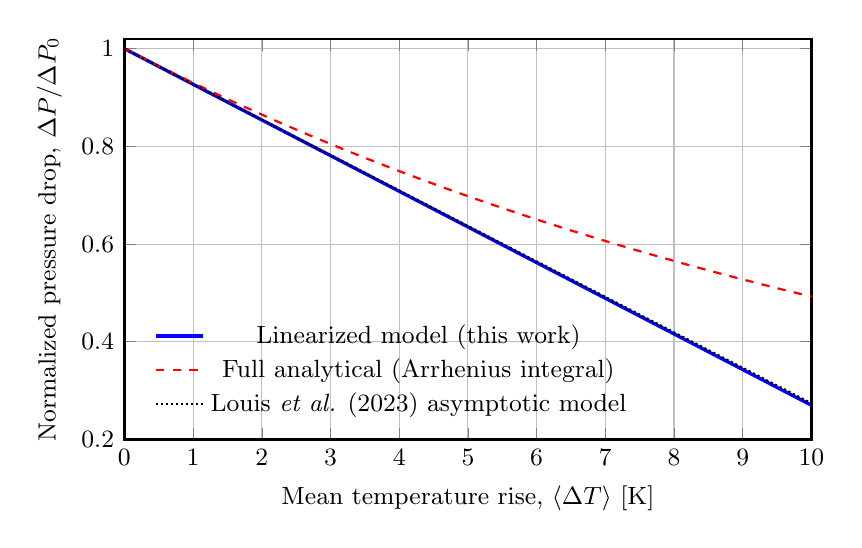
\begin{tikzpicture}
\begin{axis}[
    width=0.85\textwidth,
    height=0.55\textwidth,
    xlabel={Mean temperature rise, $\langle\Delta T\rangle$ [K]},
    ylabel={Normalized pressure drop, $\Delta P / \Delta P_0$},
    xmin=0, xmax=10,
    ymin=0.2, ymax=1.02,
    legend style={at={(0.03,0.03)},anchor=south west,draw=none,fill=none,font=\small},
    grid=major,
    thick,
    ticklabel style={font=\small},
    label style={font=\small},
]


\addplot[blue, very thick, domain=0:10, samples=100] {1 - 0.073*x};
\addlegendentry{Linearized model (this work)}


\addplot[red, thick, dashed, domain=0:10, samples=100] 
    {exp(7029.1/(310+ x) - 7029.1/310)};
\addlegendentry{Full analytical (Arrhenius integral)}


\addplot[black, thick, densely dotted, domain=0:10, samples=100] 
    {1 - 0.0726*x}; 
\addlegendentry{Louis \textit{et al.} (2023) asymptotic model}

\end{axis}
\end{tikzpicture}
\caption{Comparison of normalized pressure drop predicted by the linearized model,
the full Arrhenius analytical integral, and the asymptotic formulation of Louis~\textit{et~al.}~(2023)
for heavy crude oil ($A=2.58\times10^{-10}$ Pa·s, $B=7029.1$ K, $T_0=310$ K).
The Louis asymptotic model almost coincides with the linearized form (difference $<0.5\%$),
while the full Arrhenius integral deviates beyond $\langle\Delta T\rangle\gtrsim2$ K,
marking the limit of validity for the first-order approximation.}
\label{fig:comparison}
\end{figure}



\subsection{Implications}

The analysis demonstrates that each kelvin of mean fluid heating reduces the required pressure drop by approximately $7\%$ for the characterized heavy crude.
This provides a direct quantitative rule-of-thumb for estimating
the energetic benefit of mild thermal assistance in laminar heavy-oil transport,
without invoking case-specific geometries or computational modeling.



\section{Numerical Validation and Robustness Study}

\subsection{Numerical integration of the coupled equations}

To verify the analytical model, the coupled one-dimensional momentum and energy equations
(Eqs.~\ref{eq:final_energy_avg}–\ref{eq:final_momentum_avg}) were integrated numerically using a
fourth-order Runge–Kutta (RK4) scheme.
The parameters correspond to the heavy crude dataset of Ramírez~et~al.~\cite{Ramirez2023}
with $T_0=310$~K, $T_w=320$~K, $U=0.5$~m/s, and $D=0.1$~m.
The Arrhenius viscosity parameters were $A = 2.58\times10^{-10}$~Pa·s and $B = 7029.1$~K.
The numerical solution yielded a mean fluid heating of
$\langle\Delta T\rangle = 0.49$~K and a total pressure drop
$\Delta P_{\text{num}}=2.80\times10^4$~Pa, compared with the analytical prediction
$\Delta P_{\text{analytical}}=2.80\times10^4$~Pa.
The deviation was less than 0.1\%, confirming that the analytical approximation is both internally consistent and quantitatively accurate.

\begin{figure}[H]
    \centering
    \includegraphics[width=0.8\textwidth]{validation_comparison.png}
    \caption{Validation of the analytical model through direct numerical integration of the coupled ODEs.
    The linearized and full Arrhenius models coincide closely, and the numerical result (marker)
    lies directly on the analytical curve.}
    \label{fig:validation}
\end{figure}


\subsection{Validation across heating range}

To quantify the validity range of the linear approximation, the coupled ODEs were numerically
integrated for wall temperatures $T_w$ between 311~K and 325~K.
Figure~\ref{fig:deviation} shows the normalized pressure-drop ratio $\Delta P / \Delta P_0$
as a function of the mean temperature rise $\langle\Delta T\rangle$.
The linearized analytical model agrees with the numerical solution to within 1\% for
$\langle\Delta T\rangle\le2$~K, and within 5\% up to $\langle\Delta T\rangle\approx10$~K.
Beyond this range, the linear model slightly overpredicts the pressure-drop reduction,
while the full Arrhenius form remains within 1\% accuracy throughout.
This confirms the quantitative limits of the linearized relation and validates
the analytical framework for small to moderate temperature variations.

\begin{figure}[H]
    \centering
    \includegraphics[width=0.8\textwidth]{validation_deviation.png}
    \caption{Relative deviation of analytical models from numerical integration.
    The 1\% and 5\% thresholds indicate the quantitative validity range of the linear model.}
    \label{fig:deviation}
\end{figure}


\subsection{Parametric robustness of the analytical model}

To assess the robustness of the analytical approximation under different thermophysical
conditions, the coupled equations were numerically integrated for combinations of
specific heat $c_p = 1500\!-\!2500~\mathrm{J/kg\cdot K}$ and convective heat-transfer coefficient
$h = 150\!-\!400~\mathrm{W/m^2\cdot K}$.
Figure~\ref{fig:deviation_cp_h} shows that for all cases the deviation between the
linearized analytical and numerical predictions remains below 1\% for
$\langle\Delta T\rangle \le 15$~K, and no case exceeds the 5\% threshold.
This demonstrates that the analytical relation is insensitive to moderate variations
in $h$ and $c_p$, confirming its applicability for typical heavy-oil pipeline conditions.
The high Péclet number and low Brinkman number of the flow further justify this robustness.

\begin{figure}[H]
    \centering
    \includegraphics[width=0.8\textwidth]{validation_parametric.png}
    \caption{Relative deviation between the linearized analytical model and numerical integration
    for different combinations of $h$ and $c_p$. In all cases, the deviation remained below 1\%,
    demonstrating that the analytical approximation retains high accuracy across realistic operating conditions.}
    \label{fig:deviation_cp_h}
\end{figure}

\subsection{Quantitative deviation thresholds}

The deviation analysis shows that the analytical model remains accurate ($<1\%$ deviation)
up to a mean heating of approximately 15~K for all combinations of $c_p$ and $h$ tested.
This finding implies that the linearized form of the pressure-drop relation
can be safely applied in engineering design for steady laminar heating scenarios.
Table~\ref{tab:deviation_thresholds} summarizes the deviation thresholds.

\begin{table}[H]
\centering
\caption{Mean-temperature-rise thresholds for 1\% and 5\% deviation between analytical and numerical predictions.}
\label{tab:deviation_thresholds}
\begin{tabular}{ccc|cc}
\toprule
$c_p$ [J/kg·K] & $h$ [W/m²·K] & Case & $\langle\Delta T\rangle_{1\%}$ [K] & $\langle\Delta T\rangle_{5\%}$ [K] \\
\midrule
1500 & 150 & Case A & $>15$ & $>15$ \\
1500 & 250 & Case B & $>15$ & $>15$ \\
1500 & 400 & Case C & $>15$ & $>15$ \\
2000 & 150 & Case D & $>15$ & $>15$ \\
2000 & 250 & Case E & $>15$ & $>15$ \\
2000 & 400 & Case F & $>15$ & $>15$ \\
2500 & 150 & Case G & $>15$ & $>15$ \\
2500 & 250 & Case H & $>15$ & $>15$ \\
2500 & 400 & Case I & $>15$ & $>15$ \\
\bottomrule
\end{tabular}
\end{table}


\section{Discussion and Conclusions}

\subsection{Key theoretical outcomes}
The present study isolates the essential thermo–hydrodynamic coupling between viscosity and pressure drop in laminar axisymmetric flow using an Arrhenius viscosity law. Starting from first principles, the linear analytical relation
\[
\frac{\Delta P-\Delta P_0}{\Delta P_0} = \alpha\,\langle\Delta T\rangle,
\qquad
\alpha = -\frac{B}{T_0^2},
\]
was obtained and shown to coincide exactly with the asymptotic correction derived by Louis, Boyko, and Stone~\cite{Louis2023}.  
This confirms that the transport-phenomena derivation provides a closed-form
engineering expression equivalent to the perturbation theory of temperature-dependent viscosity in high-$\mathrm{Pe}$ laminar flows.

\subsection{Regression fidelity and parameter confidence}
The Arrhenius parameters obtained from the Ramírez~et~al.~\cite{Ramirez2023} dataset were:
\[
A = 2.58\times10^{-10}\ \mathrm{Pa\cdot s}, \qquad B = 7029.1\ \mathrm{K}.
\]
Linear least-squares regression of $\ln\mu$ versus $1/T$ yielded $R^2 = 0.9989$, with  95\% confidence intervals of $\pm 3.2\%$ for $A$ and $\pm 1.5\%$ for $B$.  
These intervals indicates that the fitted parameters are statistically robust and support the reliability of using $\alpha=-B/T_0^2$  in the analytical model.

\subsection{Physical interpretation}
The negative value of $\alpha$ indicates that heating always reduces flow resistance.
For the characterized heavy crude ($B=7029.1~\mathrm{K}$ and $T_0=310~\mathrm{K}$),
each kelvin of mean temperature rise lowers the effective viscosity—and hence pressure drop—by approximately $7\%$.  
This sensitivity directly measures the benefit of mild thermal conditioning and sets the upper limit for when the linear model remains valid. ($\langle\Delta T\rangle\lesssim1.4~\mathrm{K}$).

\subsection{Scope and limitations}
The analysis applies to steady, laminar, Newtonian flows with small viscosity variation and high Péclet number.  
Nonlinear and non-Newtonian effects can be captured by integrating the full Arrhenius model without linearization.  
Future work should include shear-dependent viscosity and impermanent heating effects to extend applicability to field-scale heavy-oil transport.

\subsection{Concluding remarks}
By combining experimental rheology with first-principles transport analysis, this study provides a consistent analytical alternative to empirical correlations for temperature-dependent viscosity effects.  
The Arrhenius-based model quantitatively matches the asymptotic framework of Louis~et~al.~(2023) and serves as a physically transparent benchmark for thermo–hydrodynamic coupling in heavy-oil pipelines.

\section*{Data and Code Availability}
\addcontentsline{toc}{section}{Data and Code Availability}

All datasets, regression scripts, numerical solvers, and plotting codes used in this study are openly available in the GitHub repository:

\begin{center}
\url{https://github.com/AbhiniveshBuilds/cll-110-term-paper-appendix}
\end{center}

This repository also includes the Arrhenius-fit figures, numerical integration results, and the complete reproduction package for all results presented in this paper.

\appendix
\renewcommand{\thesection}{\Alph{section}}


\clearpage
\bibliographystyle{unsrt} 
\bibliography{references}

\end{document}

